\documentclass{article}

\usepackage[nonatbib]{nips_2017}
\usepackage{nips_2017}

% to compile a camera-ready version, add the [final] option, e.g.:
% \usepackage[final]{nips_2017}

\usepackage[utf8]{inputenc} % allow utf-8 input
\usepackage[T1]{fontenc}    % use 8-bit T1 fonts
\usepackage{hyperref}       % hyperlinks
\usepackage{url}            % simple URL typesetting
\usepackage{booktabs}       % professional-quality tables
\usepackage{amsfonts}       % blackboard math symbols
\usepackage{nicefrac}       % compact symbols for 1/2, etc.
\usepackage{microtype}      % microtypography
\usepackage{graphicx}

\usepackage[backend=biber]{biblatex}
\addbibresource{NIPS2017.bib}
\DeclareLanguageMapping{english}{american-apa}

\title{Combining intrinsic motivation and hierarchical reinforcement learning}

\author{
  Maria K.~Eckstein \\
  Department of Psychology \\
  UC Berkeley \\
  Berkeley, CA 94720 \\
  \texttt{maria.eckstein@berkeley.edu} \\  
  \And
  Anne GE Collins \\
  UC Berkeley \\
  Address \\
  \texttt{annecollins@berkeley.edu} \\
}

\begin{document}

\maketitle

\begin{abstract}
    Humans have the astonishing ability to acquire representations of their environment that allow them to learn from little and unorganized data often sparse in rewards, and to create multi-step goal-directed action plans in computationally efficient ways. How humans achieve this has fascinated researchers in psychology as well as artificial intelligence. We suggest that the combination of two specific mechanisms contributes to this ability: curiosity, the intrinsic motivation to explore novel states; and hierarchical structure, the representation of problems and actions across multiple levels of abstraction. In order to test this hypothesis, we created a curiosity-driven hierarchical reinforcement learning agent (CHRL) and let it explore an unknown environment with hierarchical structure and no rewards. The results are promising: CHRL learns to perform meaningful action sequences of increasing length, at fixed computational cost. This allows CHRL to explore the environment more systematically than agents that lack curiosity, hierarchical structure, or both; to discover a larger number of meaningful states; and to visit these states more often. In future research, we will compare the performance of human participants in this task to CHRL's, validate and improve the model, and identify the neural substrates underlying these mechanisms in the human brain.
\end{abstract}


\section{Introduction}

Previous research in the cognitive sciences has revealed two mechanisms that are crucial for fast, efficient learning and for flexible, goal-oriented behavior: the guidance of exploration by intrinsic motivation \cite{gopnik_scientific_2012, schmidhuber_formal_2010, lepper_undermining_1973, pathak_curiosity-driven_2017}; and the hierarchical structure of representations \cite{collins_reasoning_2012, anderson_act:_1996, miller_integrative_2001, frank_mechanisms_2012, chase_perception_1973, botvinick_model-based_2014}. Here, we argue that these two mechanisms go hand in hand, such that intrinsic motivation plays a role in learning hierarchical representations. One argument for this comes from neuroscience: Midbrain dopaminergic activity, known to be elicited by reward prediction errors \cite{schultz_neural_1997} and to act as a learning signal for the brain, is also elicited by novel events \cite{wittmann_striatal_2008}, suggesting that novelty too might trigger learning, by ways of curiosity and intrinsic motivation.

In this paper, we propose a curiosity-driven hierarchical reinforcement learning (CHRL) algorithm that explores a rewards-free environment based on its intrinsic curiosity. Once a novel event elicits the agent's curiosity (like an infant playing with a toy that suddenly makes a new sound), the agent will try to reproduce the event (the new sound). Crucially, the agent does not know yet how to produce the event that it is curious about. In order to achieve its goal, it has to learn, through trial and error, a specific option policy that leads to the event \cite{sutton_between_1999}. Creating multiple such option policies, targeted at multiple different events, the agent will over time learn to control the behavior of its environment. Similar ideas have recently been proposed by others \cite{machado_learning_2016, chentanez_intrinsically_2005, pathak_curiosity-driven_2017, kulkarni_hierarchical_2016}.

Crucially in our framework, option policies can be used as building blocks for more abstract option policies, such that over time, CHRL creates a hierarchical model of its environment in terms of action plans. CHRL can reuse previously acquired option policies to achieve more complex goals, and structure its exploration into self-selected goals, sub-goals, sub-sub-goals, etc. It thereby relies solely on internally determined learning signals: 1) for learning option policies, an internal pseudo-reward upon achieving its self-selected goal; and 2) the events' novelty for learning the value of options.

In the following, we show that CHRL outperforms other agents in a simple hierarchical environment. It explores the environment both more efficiently (visiting a larger number of distinct states) and more deeply (producing a larger number of abstract events). CHRL even produces more events than agents that are directly maximizing the number of produced events. This shows that the hierarchical representation CHRL acquires of the task allows for meaningful behavior even in the absence of rewards. 

\section{Methods}

\subsection{The MDP}

We created a learning environment with a hierarchical structure similar to more naturalistic tasks such as language or motor learning, which could also be presented to humans.
In the task, the agent executes basic actions that deterministically trigger basic ("level-0") events. Applied to the example of language, the agent is initially able to produce individual phonemes. In the task, certain sequences of basic actions trigger additional "level-1" events. In the case of language, sequences of phonemes create syllables. Similarly, certain sequences of level-1 events produce level-2 events, like the combination of syllables creates words, words create sentences, etc.

Formally, we define the set of the agent's $k_0$ basic actions $\mathcal{A}_0 = \{a_{0, 1}, a_{0, 2}, \ldots, a_{0, k_0}\}$. We define each element of the state space $\mathcal{S}$ as the tuple $(f_{0, 1}, \ldots, f_{0, k_0}, \ldots, f_{L, 1}, \ldots, f_{L, k_L})$, defined by binary features $f_{l, i}$ for levels $l$ and index $i$. When the agent selects $a_{0,i}$ at trial $t$, the new state's level-0 features are $f_{0,i}=1$ and $\forall j \neq i, f_{0,j}=0$: action $a_{0, i}$ elicits "event" $e_{0, i}$, a changes in the feature $f_{0, i}$ from 0 to 1. Furthermore, at any level $l$, there is at most one index $i$ such that $f_{l,i}=1$: all features $f_{l, j}, \forall j\neq i$ are set to $0$ before feature $f_{l, i}$ is set to $1$. Last, at each level $l$, there exist triplets $i \neq j$ and $k$ such that if $f_{l,i}(t)=1$ and $a(t)=a_{l,j}$, then $f_{l+1, k}=1$: lower-level actions in specific states can trigger higher-level events, in addition to their own level's event.

\subsection{Event novelty and curiosity}

CHRL explores the environment based on its curiosity. Curiosity is determined by event novelty and determines the agent's propensity to select an event as a target of exploration. Formally, novelty of event $e$ is defined as $n_e = e^{-\lambda i_e}$ where $i_e$ is the number times event $e$ has occurred since the agent's first encounter with the environment and $\lambda$ is the agent's rate of novelty decay. We assume that curiosity $c_e$ about an event is learned through reinforcement, with delay-discounted novelty serving as teaching signal: $c_e(t+1) = c_e(t) + \alpha (\gamma^{j_e} n_e(t) - c_e(t))$ whenever event $e$ occurs. Here, $\alpha$ is the agent's learning rate; $\gamma$ is the agent's discounting of the future, and $j_e$ is the number of time steps spent within option $o_e$, which led to event $e$ ($j_e = 0$ when event $e$ happened without executing option $o_e$; $j_e = 1$ when $e$ is a basic event). In order to select specific events as sub-goals, the agent uses $\epsilon$-greedy selection based on its curiosity.

\subsection{Option creation}

Initially, the agent can only execute basic actions. When a higher-level event occurs for the first time, it is added to the agent's option set as a potential sub-goal. The option policy of the new sub-goal can use all options at the level below to reach the new sub-goal. We use the options framework to formulate CHRL's options \cite{sutton_between_1999}. The agent's initial option set $\mathcal{O}$ comprises only basic actions, $\mathcal{O} = \mathcal{A}_0$. When event $e_{l, i}$ occurs for the first time, the agent's option set is extended by the option $o_{e_{l, i}}$ targeted at producing event $e_{l, i}$: $\mathcal{O} = \mathcal{O} \cup o_{e_{l, i}}$. Each option's initiation set $\mathcal{I}$ is the whole state space, $\mathcal{I} = \mathcal{S}$. The termination condition $\beta: \mathcal{O} \rightarrow [0, 1]$ is the following. An option terminates with probability $\beta=1$ at all states in which $f_e = 1$ (in which the target event $e$ occurred) and with $\beta = \epsilon_T$ in all other states. The action set of option $o_{e_{l, i}}$ at level $l$ comprises all options $o_{e_{l-1, \cdot}}$ at level $l-1$. For example, the policy of a level-1 option $o_1$ operates on the action space comprising all basic actions $a_{0, i} \in \mathcal{A}_0$. 

\subsection{Learning option policies}

When the agent selects a specific event $e$ as sub-goal, the option policy $o_e$ controls action selection until option $o_e$ terminates. The option policy learns through temporal-difference learning \cite{sutton_reinforcement_2017} which actions lead to the sub-goal. After option termination, the agent's curiosity about the sub-goal is updated based on the novelty of the produced event (or the failure to produce the event).

%Formally, option $o$'s policy $\pi_o$ is $\epsilon$-greedy over within-option values $V_o$. $V_o$ are defined by the weights $\theta$ of the binary features $f(t)$ that describe the state of the environment at time $t$, $V_o^{t}(s_t, a_t) = \theta^T f^t$. 
%$V_o$ are updated through temporal difference learning on the weights $\theta$: $\theta^{t+1} = \theta^t + \alpha (r_p + \gamma \max_a(V_o^{t}(s^{t+1}, a)) - V_o^{t}(s^t, a^t))$; here, the pseudo-reward $r_p = 1$ when $e$ occurred (and the option terminates) and $r_p = 0$ otherwise; $V_o(s^{t+1},\cdot) = 0$ when the option terminates. 


\section{Results}

\subsection{Simulations and competing algorithms} \label{Comparison agents}

We simulated CHRL's behavior over environments designed to be sufficiently complex to challenge learning: $5$ hierarchical levels of $5$ events per level. All higher-level events were triggered by sequences of two subsequent events at the level directly below.%; rules were allowed to overlap, but could not be identical, e.g., when one rule was $e_{l_2} + e_{l_3} \rightarrow e_{l+1, 1}$ ($e_{l_2}$ followed by $e_{l_3}$ produces $e_{l+1, 1}$), another rule might be $e_{l_2} + e_{l_4} \rightarrow e_{l+1, 2}$). 

Agents explored the environment for 400 time steps, i.e., executing 400 basic actions. We used the following parameter settings for all agents: $\alpha = 0.3$, $\lambda = 0.3$, $\gamma = 0.9$, $\epsilon = 0.2$, and $\epsilon_T = 0.1$. We obtain similar results with different parameter sets. The data shown below are based on the average performance of 99 agents in a single environment (section \ref{Results CHRL}), and the average performance of 3 agents in 15 environments (section \ref{Results compare all}). The results hold for individual agents and environments.

To investigate the importance of both hierarchical structure and novelty seeking to behavior, we compared CHRL to three other agents without one or both of these mechanisms. Reward-based agents used a reward function defined as the number of current events instead of novelty; flat agents did not create options.%The reward-based hierarchical agent created and employed options in the same way as the CHRL agent, but used reward $r$ instead of novelty as an update signal for option values; we define reward as the number of events produced in a given trial.
%The novelty-based flat agent selected options based on curiosity like the CHRL agent, but it did not create or use options. Therefore, $O = A_0$ and $S = S_0$. The reward-based flat agent is a combination of these two agents, with neither options nor novelty-based learning.

\subsection{Behavior of the CHRL agent} \label{Results CHRL}

Through exploration and experience of novel events, CHRL acquires several hierarchically structured option policies. Option policies targeted at simpler events were learned faster than the ones targeted at more abstract events (data not shown).

In addition, the agent's curiosity decreased faster for less abstract events than for more abstract events (fig. \ref{CuriosityFigure}). In other words, the simpler an option, the faster the agent lost interest in executing it for its own sake. Importantly, this does not imply that the agent executed all less abstract options less often: on the contrary, the rate of even the simplest options increased over time (fig. \ref{CEvents}). This is because simple options form the building blocks of all abstract options.

\begin{figure}[h]
	\centering
	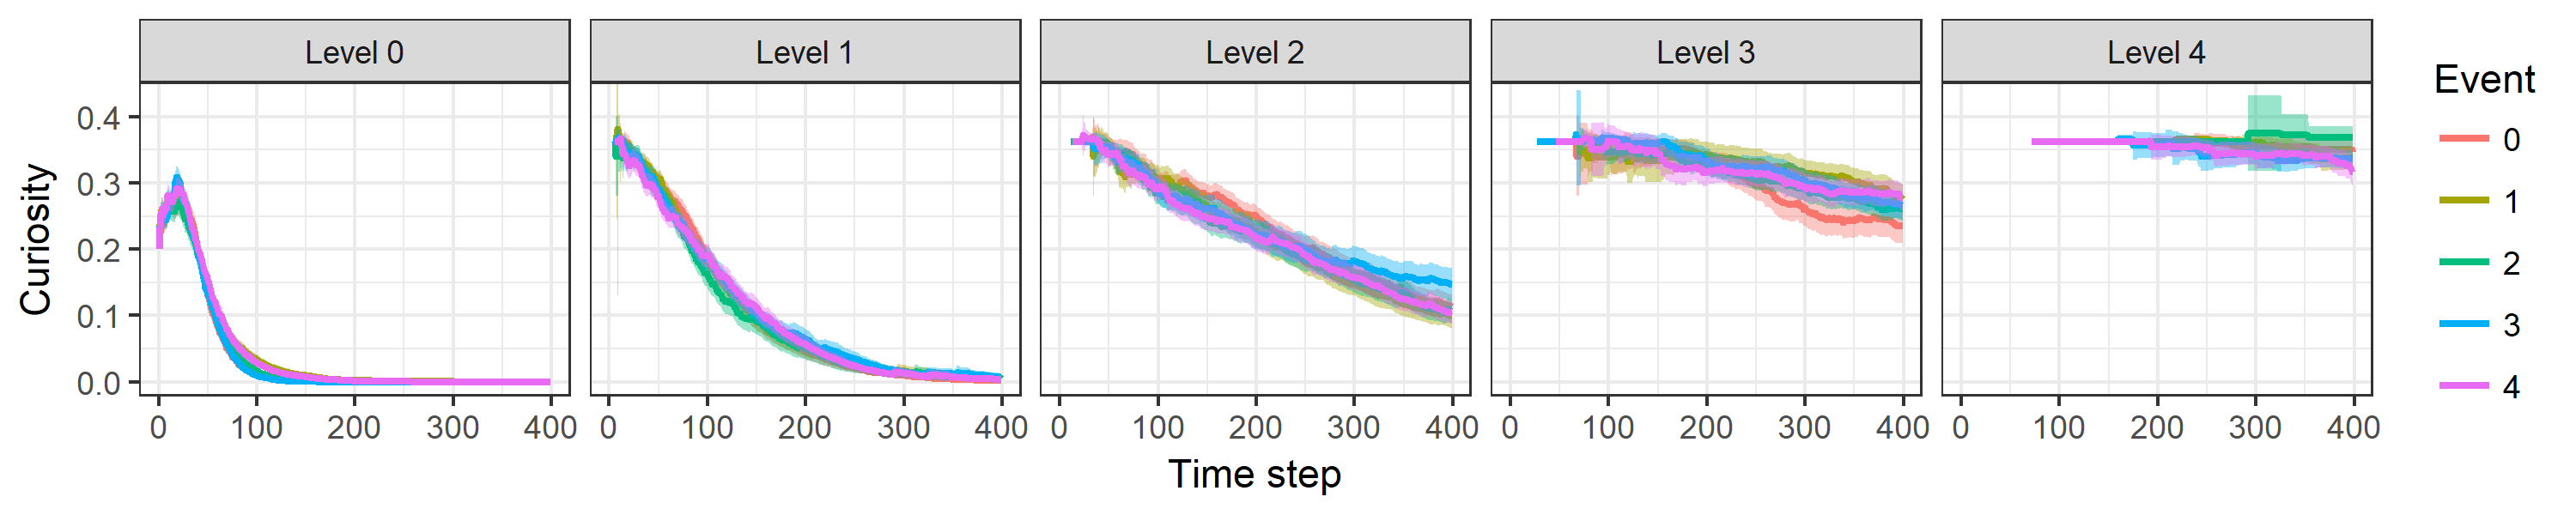
\includegraphics[width=\linewidth]{ACuriosity.png}
	\caption{Curiosity for events decreases over time. Shaded areas indicate 95\% confidence intervals of the mean. The higher-level an event, the slower curiosity decreases.}
	\label{CuriosityFigure}
\end{figure}

\subsection{Comparison of CHRL and other agents} \label{Results compare all}

We compared CHRL's behavior to three other agents (see section \ref{Comparison agents}). CHRL discovered a larger number of different events than the other agents, and at a faster rate (fig. \ref{CEvents}A). The reward-based flat agent was outperformed by both the novelty-based flat agent and the reward-based hierarchical agent, suggesting that both curiosity and hierarchical structure were crucial for effective exploration.

The reason for the exploration advantage is that CHRL's curiosity is larger for more abstract events because these are more difficult to obtain, and therefore remain more novel. Due to that, CHRL will execute more higher-level options (fig. \ref{CEvents}B), which increases the probability of observing events at higher levels. 

\begin{figure}[h]
	\centering
	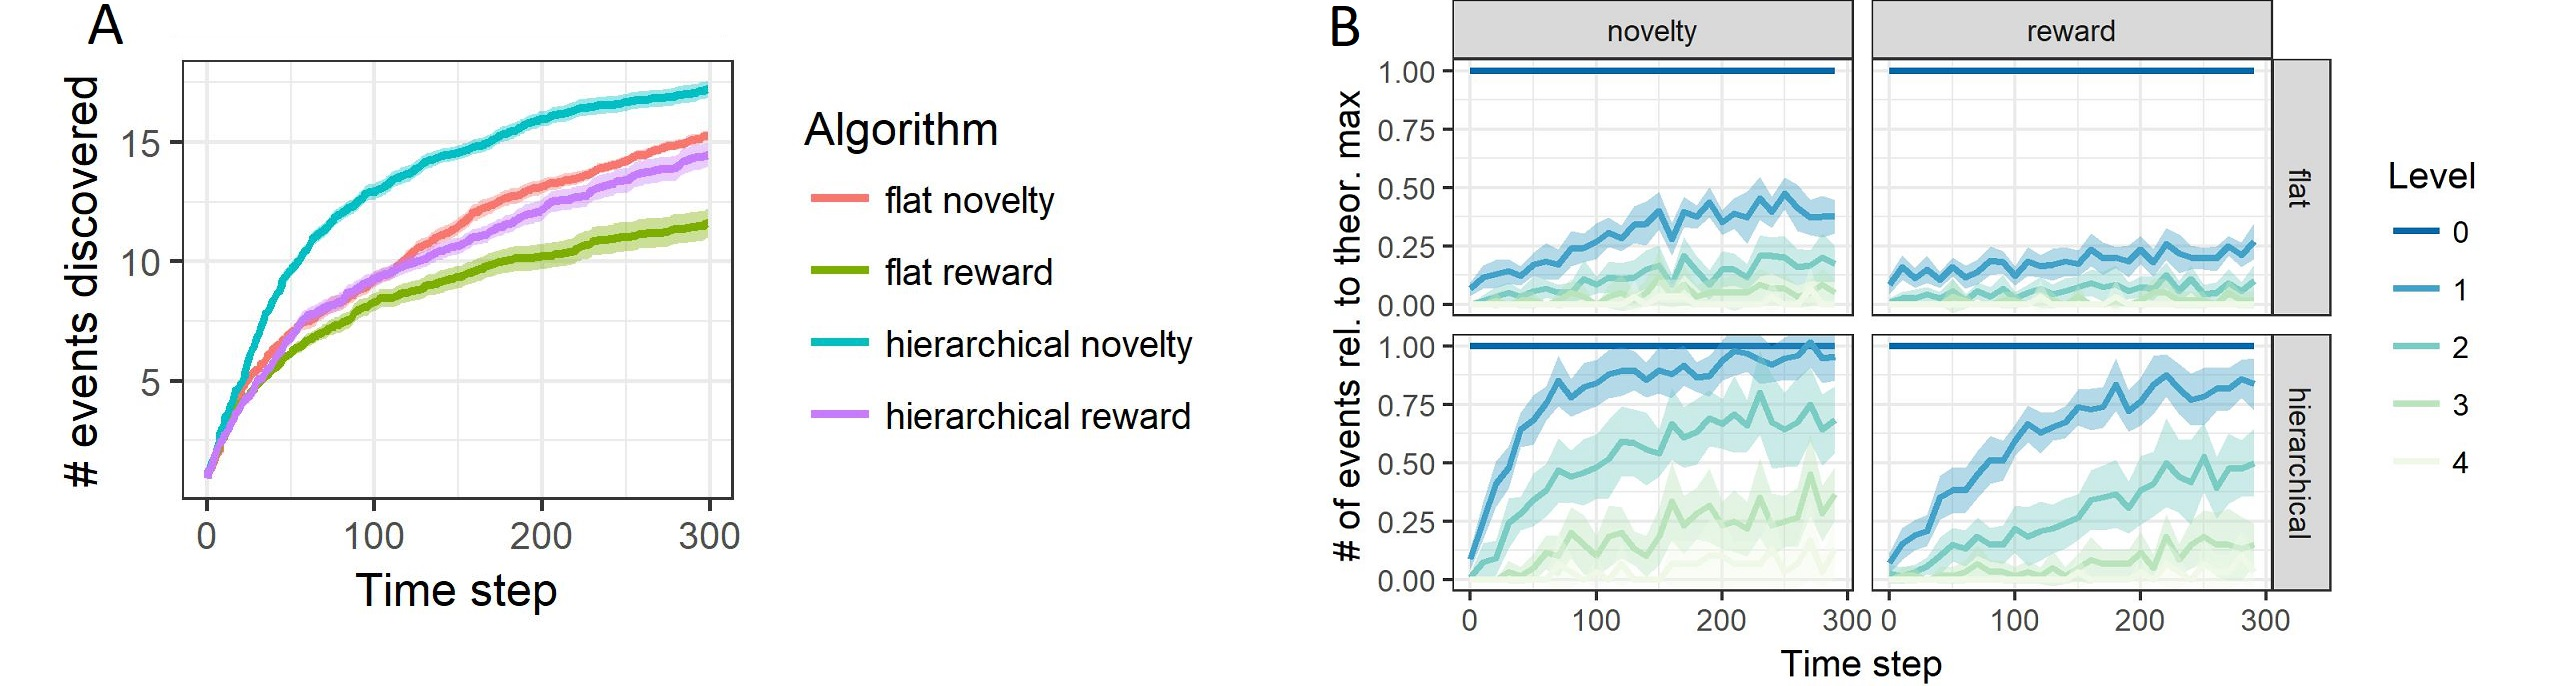
\includegraphics[width=\linewidth]{CEvents.jpg}
	\caption{A) Number of events discovered by each agent. B) Number of events that occurred in each bin of 20 time steps, relative to theoretical maximum (theor. max. for level-0: 20 / 20; level-1: 10 / 20; level-2: 5 / 20; etc.). Shaded areas indicate 95\% confidence intervals of the mean.}
	\label{CEvents}
\end{figure}

\section{Conclusion}

We hypothesized that two factors crucially contribute to human ability to form goal-directed, abstract action plans in environments that are unorganized and sparse in rewards: curiosity-driven exploration and the creation of hierarchical option policies. Both factors have been the target of various research in the cognitive sciences and, more recently, have gained interest in computer science and artificial intelligence research \cite{botvinick_model-based_2014, frank_mechanisms_2012, gopnik_scientific_2012, machado_learning_2016, anderson_act:_1996, collins_reasoning_2012, miller_integrative_2001, schmidhuber_formal_2010, pathak_curiosity-driven_2017, kulkarni_hierarchical_2016}.

In order to test this hypothesis, we implemented CHRL, a reinforcement-learning algorithm that is driven by curiosity and that has the ability to create hierarchical option policies. This agent indeed shows characteristics expected from human learners. For example, the agent's curiosity declines fastest for basic events, but slower for more abstract events. This is because option policies become better and better at producing their goal events, such that the corresponding events occur more frequently and, over time, decrease in novelty. This leads to a decrease in the agent's intrinsic motivation to explore events further once they are understood. Nevertheless, this process does not slow down learning: Acquiring new skills, rather than reducing motivation, opens up new possibilities of learning even more abstract skills. Similarly, in the human domain, whereas an infant might be curious about individual sounds, a toddler might be interested in children's songs, and an adult in twelve-tone music or Italian Opera. 

To confirm the importance of both mechanisms, we compared CHRL to flat and reward-driven agents. CHRL outperforms the other agents in terms of exploration efficiency, discovering a larger number of different events in the given environment. It also produces an overall larger number of abstract events than the other agents. This is especially remarkable because other agents are rewarded based on the number of events they triggered, whereas CHRL was not. This highlights how powerful novelty can be as a learning signal.

%Because we focus on understanding human intelligence rather than  artificial intelligence, we have not yet compared our agent to other option creation schemes. Nevertheless, it will be important in future research to compare our framework to others. It would be especially exciting to integrate advances from this field, such as curiosity based on prediction rather than counting. 

Our algorithm assumes simple mechanisms for detecting events and measuring novelty. Although this limits the usefulness of the algorithm in complex AI problems, it is advantageous for our research because it maximizes experimental control. Once translated into a human task, we will be able to explore how several factors contribute to hierarchical learning, such as the number of basic actions, the length of options, and the depth of environmental hierarchy (number of levels). 

Our goal for future work is to adjust the algorithm to capture human behavior in this task, reproducing the overall pattern as well as typical mistakes. An algorithm with human-like behavior will allow us to study the neural underpinnings of the mechanisms underlying curiosity-based exploration and hierarchical structure. It might also inform AI research by providing insights into human reasoning in a complex domain.

In summary, by creating the hierarchical novelty-seeking agent, we showed that learning of meaningful behavior can be driven by learning itself, rather than external rewards. In this framework, the learner produces the crucial learning signals itself, by selecting actions that over time reduce novelty. In other words, this learner balances the search for novelty with reducing prediction errors. It explores the environment in a systematic way, forms "hypotheses" and conducts "experiments", in order to learn more, just like is expected from a human learner.

\printbibliography

\end{document}